\section{Expanding the Traffic Light System: Contexts and Refinement}
\label{tut_expanding_traffic_light_system}

\tick{\textbf{Goals:} We apply what we learned in the previous section by introducing a context with traffic light colours and a refinement to integrate them. We will also introduce another refinement for the push buttons.}

\subsection{Data Refinement}
\label{tut_data_refinement}

We will continue the example from Section~\ref{tut_first_machine}, where we built a simplified model of a traffic light controller.  The model was simplified because we abstracted the traffic lights to TRUE and FALSE and a number of features were still missing.

We will introduce data refinement in this section.  The objective is to create a mapping between the abstract traffic light values and actual colours. Figure \ref{fig_tut_07_tl_colours} depicts our mapping for the traffic light.

\begin{figure}[!ht]
\begin{center}
	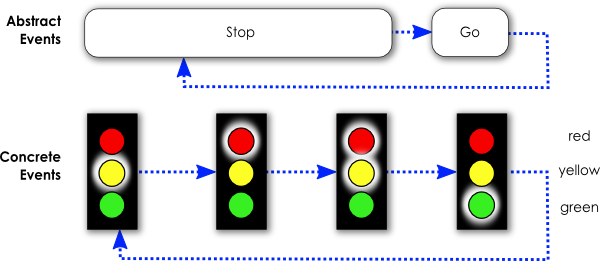
\includegraphics{img/tutorial/tl-colors.png}
	\caption{Mapping between Abstract and Concrete Events}
	\label{fig_tut_07_tl_colours}
\end{center}
\end{figure}

For simplicity, the traffic light for pedestrians consists of only two lights: red and green.

We break this problem into two steps:

\begin{enumerate}
	\item Create a context with the data structures for the colours.
	\item Create a refinement of the existing model that sees the new context and refines the boolean states into colours.
\end{enumerate}

\subsection{A Context with Colours}
\label{tut_context_with_colors}

Start by creating a context called \texttt{ctx1}, as described in Section~\ref{tut_contexts}.
We model the colours of the traffic light as a so-called ``enumerated set'' (\ref{sets}): 
We explicitly specify all elements (the three colours) of a new user-defined data type.
We define the constants:
\pencil{
\begin{description}
\CONSTANTS
	\begin{description}
		\Item{ red }
		\Item{ yellow }
		\Item{ green }
	\end{description}
\end{description}
}
We introduce the new data type as a set:
\pencil{
\begin{description}
\SETS
	\begin{description}
		\Item{ COLOURS }
	\end{description}
\end{description}
}
And last, we need to provide typing of the constants.  We do this by creating a partition (\ref{partition}):
\pencil{
\begin{description}
\AXIOMS
	\begin{description}
		\nItemX{ type }{ partition(COLOURS, \{ red\} , \{ yellow\} , \{ green\} ) }
	\end{description}
\end{description}
}

\warning{Please note the curly braces \{\} around the colours.  It's very easy to forget these, but if they are missing, a typing errors will be displayed that are hard to interpret for a novice.
}

This completes the context.

\subsection{The Actual Data Refinement}
\label{tut_actual_data_refinement}

The easiest way to create a refinement is by right-clicking on the machine in the project browser and selecting \textsf{Refine} (in this case, we will be refining the machine \textsf{mac} from the project \textsf{tutorial-3}).  This will create a ``stub'' consisting of all variables and events. Please use this method to create a machine with name \texttt{mac1}.

When you have refined a machine, the Rodin Editor will show you all the elements of the abstracted machine, but the inherited actions will be shown in grey. This means that you can add actions to the event, but you cannot edit the actions that are already there.

%\warning{In refinements, the \textsf{Edit} View of the Editor hides some information from the abstract machine by default.  This can be particularly important when you modify a refined event.  The \textsf{Pretty Print} View shows all the element with elements from the abstract machine in \textit{italics}.}



\warning{For this tutorial, make sure that you right-click on the machine and select refine from the drop-down menu. If you have created a machine the normal way and later edited the refines section, the tutorial will assume that you have events (e.g. \textsf{sets\_peds\_go}) and variables that you do not have.  }

First we have to make the machine aware of the context by adding a \textsf{sees} (\ref{seeing_a_context}) statement. To do this, place your cursor to the left of the small green arrow next to your machine name \textsf{mac1}. Right click and select \textsf{Add Child $\rangle$ Event-B Sees Context Relationship}. A \textsf{SEES} heading will appear with the value \textsf{--undefined--}. Place your cursor over the undefined section and click. A small box listing all of the contexts in the project will pop up. Select \textsf{ctx1}:

\pencil{
\begin{description}
\MACHINE{mac1}
\REFINES{mac}
\SEES{ctx1}
\end{description}
}

We will start with the traffic lights for the pedestrians. It has only two colours (red and green) and only one of them is shown at a time.  We introduce a new variable called \textsf{peds\_colour} to represent which of the lights is shown. The variable has a corresponding invariant and initialization (the changes are shown in the following code snippet). The \textit{extended}	keyword in the initialisation means that all
actions from the refined initialisation are copied:

\pencil{
\begin{description}
\VARIABLES
	\begin{description}
		\Item{ peds\_colour }
	\end{description}
\INVARIANTS
	\begin{description}
		\nItemX{ inv4 }{ peds\_colour \in  \{  red, green \}  }
	\end{description}
\EVENTS
	\INITIALISATION
		\\\textit{extended}		
		\begin{description}
		\BeginAct
			\begin{description}	
			\nItemX{ init4 }{ peds\_colour :=  red }
			\end{description}
		\EndAct
		\end{description}
\END
\end{description}
}

\index{gluing invariant}
Next, we will create a gluing invariant (\ref{abstract_machine}) that associates \textsf{peds\_go} from the abstract machine with the variable \textsf{peds\_colour} that we just created.  The gluing invariant will map \textsf{TRUE} to \textsf{green} and \textsf{FALSE} to \textsf{red}:

\pencil{
\begin{description}
\INVARIANTS
	\begin{description}
		\nItemX{ gluing }{ peds\_go = TRUE \leqv  peds\_colour = green }
	\end{description}
\end{description}
}

In its current state, this gluing invariant can be violated: if the event \textsf{set\_peds\_go} is triggered, for instance, the variable \textsf{peds\_go} will change but \textsf{peds\_colour} will not.  We expect that this will result in undischarged proof obligations (\ref{generated_proof_obligations}).  We can check this by expanding the machine in the Event-B Explorer.  Indeed, we now see two undischarged proof obligations (compare with Figure \ref{fig_tut_07_undischarged}).

\begin{figure}[!ht]
\begin{center}
	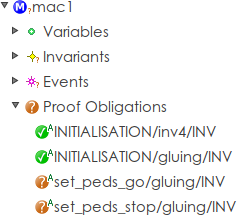
\includegraphics{img/tutorial/undischarged1.png}
	\caption{Mapping between Abstract and Concrete Events}
	\label{fig_tut_07_undischarged}
\end{center}
\end{figure}

To fix this, we have to modify the two events in question.  Let's start with \textsf{set\_peds\_go}.  First, we change the event from extended to not extended in the Editor by placing our cursor over the keyword \textsf{extended} and clicking. This is shown in Figure \ref{fig_tut_07_event_refinement}.

\begin{figure}[!ht]
\begin{center}
	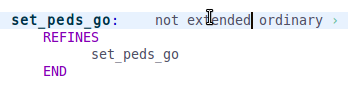
\includegraphics{img/tutorial/tut_07_event_refinement.png}
	\caption{Switch from extended to not extended}
	\label{fig_tut_07_event_refinement}
\end{center}
\end{figure}

This change will copy the guard and action from the abstract machine, so that we can modify it.  We can now replace the action with the corresponding action regarding \textsf{peds\_colour} (replacing \textsf{peds\_go := true} with \textsf{peds\_colour := green}).  While we are at it, we can also rename the name of the event to something more fitting (e.g. \textsf{set\_peds\_green}).

Next, we perform the corresponding change on \textsf{set\_peds\_stop} (change the action to \textsf{peds\_colour := red} and rename the event \textsf{set\_peds\_red}). Lastly, the event \textsf{set\_cars} also contains a reference to \textsf{peds\_go} that must be replaced (in the second guard, replace \textsf{peds\_go = FALSE} with \textsf{peds\_colour = red}).

Once all references to \textsf{peds\_go} have been replace, we can remove the variable \textsf{peds\_go} from the \textsf{VARIABLES} section. You will also need to change the \textsf{INITIALISATION} event to \textsf{not extended} and remove the action which initialises the variable \textsf{peds\_go}. Now you shouldn't have any errors or warnings, and all proof obligations should be discharged.

\warning{If you get the error message ``Identifier peds\_go has not been declared'', then there are references to the refined variable left somewhere in the model.  %It can be helpful to use the \textsf{Pretty Print} view, as it will show the ``inherited'' elements from the abstract machine as well.
}

\subsection{The refined machine with data refinement for peds\_go}
\label{tut_refined_machine}

\pencil{
\begin{description}
\MACHINE{mac1}
\REFINES{mac}
\SEES{ctx1}
\VARIABLES
	\begin{description}
		\Item{ cars\_go }
		\Item{ peds\_colour }
	\end{description}
\INVARIANTS
	\begin{description}
		\nItemX{ inv4 }{ peds\_colour \in  \{  red, green \}  }
		\nItemX{ gluing }{ peds\_go = TRUE \leqv  peds\_colour = green }
	\end{description}
\EVENTS
	\INITIALISATION
		\begin{description}
		\BeginAct
			\begin{description}
			\nItemX{ act1 }{ cars\_go :=  FALSE }
			\nItemX{ init4 }{ peds\_colour :=  red }
			\end{description}
		\EndAct
		\end{description}
	\EVT {set\_peds\_green}
	\REF {set\_peds\_go}
		\begin{description}
		\WhenGrd
			\begin{description}
			\nItemX{ grd1 }{ cars\_go = FALSE }
			\end{description}
		\ThenAct
			\begin{description}
			\nItemX{ act2 }{ peds\_colour :=  green }
			\end{description}
		\EndAct
		\end{description}
	\EVT {set\_peds\_red}
	\REF {set\_peds\_stop}
		\begin{description}
		\BeginAct
			\begin{description}
			\nItemX{ act1 }{ peds\_colour :=  red }
			\end{description}
		\EndAct
		\end{description}
	\EVT {set\_cars}
	\REF {set\_cars}
		\begin{description}
		\AnyPrm
			\begin{description}
			\ItemX{ new\_value }
			\end{description}
		\WhereGrd
			\begin{description}
			\nItemX{ grd1 }{ new\_value \in  BOOL }
			\nItemX{ grd2 }{ new\_value = TRUE \limp  peds\_colour = red }
			\end{description}
		\ThenAct
			\begin{description}
			\nItemX{ act1 }{ cars\_go :=  new\_value }
			\end{description}
		\EndAct
		\end{description}
\END
\end{description}
}

\subsection{Witnesses}
\label{tut_extend_traffic_witnesses}
\index{witness}

The refinement of \textsf{set\_cars} is more difficult since the event uses a parameter (the new value for \textsf{cars\_go}).  In order to refine it, we need a witness (\ref{witness}).

A witness is to an event's parameter what a gluing invariant is to a variable: it is a mapping between the abstract parameter and the new parameter and allows the abstract parameter to disappear.  In this example, the abstract parameter \textsf{new\_value} is of type \textsf{BOOL}, and we introduce a new parameter \textsf{new\_value\_colours} of type \textsf{COLOURS}.

\warning{The naming of a witnesses' label is extremely important. It must be the name of the abstract parameter.  In our example, the label must be \textsf{new\_value}}

Let's get started.  We first provide the new variable, gluing invariant, typing invariant and initialisation as we have done before (at this point you can also rename the gluing invariant from the last section as \textsf{gluing\_peds} in order to be able to determine between the two gluing invariants).  Note that the traffic light for the cars can show more than one colour at a time.  Therefore, the variable contains a set of colours instead of just one colour (as modelled for \textsf{peds\_colour}):

\pencil{
\begin{description}
\VARIABLES
	\begin{description}
		\Item{ cars\_colours }
	\end{description}
\INVARIANTS
	\begin{description}
		\nItemX{ inv5 }{ cars\_colours \subseteq  COLOURS }
		\nItemX{ gluing\_cars }{ cars\_go = TRUE \leqv  green \in  cars\_colours }
	\end{description}
\EVENTS
	\INITIALISATION
		\begin{description}
		\BeginAct
			\begin{description}
			\nItemX{ init5 }{ cars\_colours :=  \{  red \}  }
			\end{description}
		\EndAct
		\end{description}
	\END
\end{description}
}

We also have to modify the guard on \textsf{set\_peds\_green}, which is something that you should now be able to figure out yourself (just replace \textsf{cars\_go = FALSE} with \textsf{green} $\notin$ \textsf{cars\_colours}).

The interesting piece is the last event, \textsf{set\_cars}, which we rename as \textsf{set\_cars\_colours}.  We change the parameter to \textsf{new\_value\_colours} and type it as a subset of \textsf{COLOURS}.

The witness appears in the \textsf{with} section of the event.  The label \textbf{must} be \textsf{new\_value}.  The value itself must describe the relationship between the abstract parameter \textsf{new\_value} and the new parameter \textsf{new\_value\_colours}.  As we use the parameter as the new value for the variable \textsf{cars\_colours}, the witness is an adaptation of the gluing invariant (we just replace \textsf{cars\_colours} with \textsf{new\_value\_colours}).

\info{In most cases, the witness is a slightly modified gluing invariant.}

Here is the resulting event:

\pencil{
\begin{description}
	\EVT {set\_cars\_colours}
	\REF {set\_cars}
		\begin{description}
		\AnyPrm
			\begin{description}
			\ItemX{ new\_value\_colours }
			\end{description}
		\WhereGrd
			\begin{description}
			\nItemX{ grd1 }{ new\_value\_colours \subseteq  COLOURS }
			\nItemX{ grd2 }{ green \in  new\_value\_colours \limp  peds\_colour = red }
			\end{description}
		\Witnesses
			\begin{description}
			\nItem{ new\_value }{ new\_value = TRUE \leqv  green \in  new\_value\_colours }
			\end{description}
		\ThenAct
			\begin{description}
			\nItemX{ act1 }{ cars\_colours :=  new\_value\_colours }
			\end{description}
		\EndAct
		\end{description}
\end{description}
}

Now you can get rid of the variable \textsf{cars\_go} and its inisialisation clause, and there will not be any errors or warnings. But even though all proof obligations are now discharged, we're not done yet. Even though the traffic light doesn't violate the safety property from the abstract machine, it doesn't behave the way described in Section~\ref{tut_data_refinement}.  We still have to ensure that the lights are activated in the proper sequence.  We can impose this behavior by adding four guards each of which define one transition:

\pencil{
\begin{description}
\nItemX{ grd\_y\_r }{ cars\_colours = \{  yellow \}  \limp  new\_value\_colours = \{  red \}  }
\nItemX{ grd\_r\_ry }{ cars\_colours = \{  red \}  \limp  new\_value\_colours = \{  red, yellow \}  }
\nItemX{ grd\_ry\_g }{ cars\_colours = \{  red, yellow \}  \limp  new\_value\_colours = \{  green \}  }
\nItemX{ grd\_g\_y }{ cars\_colours = \{  green \}  \limp  new\_value\_colours = \{  yellow \}  }
\end{description}
}

\subsection{Discussion}
\label{tut_concepts_discussion}

Notice that we have used two very different approaches to model the traffic lights for cars and pedestrians.  For the pedestrians, we created one event for each state transition.  For the cars, we handled all states in one single event.

You will often be confronted with situations where many modelling approaches are possible.  You should consider two main factors when modelling: (1) the readability of the model and (2) the ease of the proof.  In this case, both approaches are equally good (although we wouldn't recommend mixing different approaches in one model. We did it here only to demonstrate both approaches).

We will cover deadlocks later in Section~\ref{deadlock}.  If you are interested in the topic, it may interest you to examine the traffic light model for deadlocks.  Consider \textsf{cars\_colours = \{ green, red \}}. This is a legal state, but it would block \textsf{set\_cars\_colours} forever.  A model checker (such as \href{http://www.stups.uni-duesseldorf.de/ProB}{ProB}) could find it.  In this case, however, this is not a problem because with the given initialization and events this state is not reachable in the first place.

We hope that this section helped you to understand the power of abstraction.  The safety invariant
$\lnot(cars\_go = TRUE \land peds\_go = TRUE)$ from Section~\ref{tutorial:invariants} was very simple.  We could now introduce colours because we are confident that the invariant will still be valid (assuming, of course, that our gluing invariant is correct).

\subsection{The Refined Machine with All Data Refinement}
\label{tut_the_refined_machine_with_all_data_refinement}

\pencil{
\begin{description}
\MACHINE{mac1}
\REFINES{mac}
\SEES{ctx1}
\VARIABLES
	\begin{description}
		\Item{ peds\_colour }
		\Item{ cars\_colours }
	\end{description}
\INVARIANTS
	\begin{description}
		\nItemX{ inv4 }{ peds\_colour \in  \{  red, green \}  }
		\nItemX{ inv5 }{ cars\_colours \subseteq  COLOURS }
		\nItemX{ gluing\_peds }{ peds\_go = TRUE \leqv  peds\_colour = green }
		\nItemX{ gluing\_cars }{ cars\_go = TRUE \leqv  green \in  cars\_colours }
	\end{description}
\EVENTS
	\INITIALISATION
		\begin{description}
		\BeginAct
			\begin{description}
			\nItemX{ init4 }{ peds\_colour :=  red }
			\nItemX{ init5 }{ cars\_colours :=  \{  red \}  }
			\end{description}
		\EndAct
		\end{description}
	\EVT {set\_peds\_green}
	\REF {set\_peds\_go}
		\begin{description}
		\WhenGrd
			\begin{description}
			\nItemX{ grd1 }{ green \notin  cars\_colours }
			\end{description}
		\ThenAct
			\begin{description}
			\nItemX{ act2 }{ peds\_colour :=  green }
			\end{description}
		\EndAct
		\end{description}
	\EVT {set\_peds\_red}
	\REF {set\_peds\_stop}
		\begin{description}
		\BeginAct
			\begin{description}
			\nItemX{ act1 }{ peds\_colour :=  red }
			\end{description}
		\EndAct
		\end{description}
	\EVT {set\_cars\_colours}
	\REF {set\_cars}
		\begin{description}
		\AnyPrm
			\begin{description}
			\ItemX{ new\_value\_colours }
			\end{description}
		\WhereGrd
			\begin{description}
			\nItemX{ grd1 }{ new\_value\_colours \subseteq  COLOURS }
			\nItemX{ grd2 }{ green \in  new\_value\_colours \limp  peds\_colour = red }
			\nItemX{ grd\_y\_r }{ cars\_colours = \{  yellow \}  \limp  new\_value\_colours = \{  red \}  }
			\nItemX{ grd\_r\_ry }{ cars\_colours = \{  red \}  \limp  new\_value\_colours = \{  red, yellow \}  }
			\nItemX{ grd\_ry\_g }{ cars\_colours = \{  red, yellow \}  \limp  new\_value\_colours = \{  green \}  }
			\nItemX{ grd\_g\_y }{ cars\_colours = \{  green \}  \limp  new\_value\_colours = \{  yellow \}  }
			\end{description}
		\Witnesses
			\begin{description}
			\nItem{ new\_value }{ new\_value = TRUE \leqv  green \in  new\_value\_colours }
			\end{description}
		\ThenAct
			\begin{description}
			\nItemX{ act1 }{ cars\_colours :=  new\_value\_colours }
			\end{description}
		\EndAct
		\end{description}
\END
\end{description}
}

\subsection{One more Refinement: The Push Button}
\label{tut_one_more_refinement}

We will demonstrate another application of refinement: introducing new features into an existing model.  A typical traffic light system allows the pedestrians to request a light change by pressing a button.  We will introduce this feature in a new refinement.

We could have introduced the push button in the initial machine, but introducing it later allows us to structure the model and makes it easier to understand and navigate.

We will realize this feature by introducing a new boolean variable for the push button.  We will introduce an event that notifies the model that a push button has been pressed.  Upon allowing the pedestrians to cross, we will reset the push button.  This is a simplification of the problem.  In practice, a lot would depend on the controller's capabilities.  We would have to consider things like how the push button notification gets to the controller software and how the pressing/depressing sequence is handled. In this example, the event directly sets the controller's state.  This demonstrates the concept of feature refinement without introducing too much complexity for a tutorial example.

As in the previous section, we create a new refinement \textsf{mac2} by right-clicking on \textsf{mac1} and selecting \textsf{Refine}.  A stub is generated that contains the events from the abstract machine.  We simply add a new variable for the push button (including typing and an initialisation clause).  We also introduce an event that sets the button.  This event doesn't work while the pedestrians have a green light.

\pencil{
\begin{description}
\VARIABLES
	\begin{description}
		\Item{ button }
	\end{description}
\INVARIANTS
	\begin{description}
		\nItemX{ type\_button }{ button \in  BOOL }
	\end{description}
\EVENTS
	\INITIALISATION
		\\\textit{extended}
		\begin{description}
		\BeginAct
			\begin{description}
			\nItemX{ init\_button }{ button :=  FALSE }
			\end{description}
		\EndAct
		\end{description}
	\EVT {push\_button}
		\begin{description}
		\WhenGrd
			\begin{description}
			\nItemX{ grd }{ peds\_colour = red }
			\end{description}
		\ThenAct
			\begin{description}
			\nItemX{ act }{ button :=  TRUE }
			\end{description}
		\EndAct
		\end{description}
	\END
\end{description}
}

Now we need to integrate the push button with the traffic light logic:
\begin{itemize}
	\item Upon pressing the button, the pedestrians must eventually get a green light.
	\item At some point, the button variable must be reset.
\end{itemize}

As we will see in the following discussion, this be more tricky than it first appears.  For now, we will introduce a guard preventing the car lights from turning green when the button is true, and we will reset the button when the pedestrian lights turn red:

\pencil{
\begin{description}
	\EVT {set\_peds\_red}
	\EXTD {set\_peds\_red}
		\begin{description}
		\BeginAct
			\begin{description}
			\nItemX{ act\_button }{ button :=   FALSE }
			\end{description}
		\EndAct
		\end{description}
	\EVT {set\_cars\_colours}
	\EXTD {set\_cars\_colours}
		\begin{description}
		\WhereGrd
			\begin{description}
			\nItemX{ grd\_button }{ \lnot  (cars\_colours = \{  red \}  \land  button = TRUE) }
			\end{description}
		\EndAct
		\end{description}
\end{description}
}

\subsection{Discussion}
\label{tut_concepts_discussion2}

There are a number of problems associated with the model in its current state.  Let's start with how the button is reset: The way we built our model so far, \textsf{set\_peds\_red} can be triggered at any time; there is not a single guard which prevents this.  Therefore, the button could be reset any time without the pedestrian light ever turning green.

This could be prevented with additional guards. For instance, the traffic light events could require an actual change in the light's status.  This in turn could lead to deadlocks.

But even if we introduce such guards, we could get stuck in a situation where cars would never get green light any more.  Consider the following scenario: (1) pedestrians get green light; (2) the light turns red; (3) a pedestrian presses the button again; (4) this prevents the car lights from turning green. Instead, the pedestrians get a green light again and the cycle continues.

There are tactics to address all these issues.  However, it is rarely possible to generate proof obligations for such scenarios (without making the model much more complicated).  It can be useful to use model checkers to validate the model's behaviour or even to use temporal logic to articulate properties of the model.

\info{As an exercise, try to improve the model to address these issues.}


%%% Local Variables: 
%%% mode: latex
%%% TeX-master: "rodin-doc"
%%% End: 
